\section{Running the SCALE-LES}
%####################################################################################

\subsection{モデル実行方法の概要}
%====================================================================================

SCALE-LESモデルの実行過程は,Fig. \ref{fig:howto}に示されるように
\begin{enumerate}
\item pp : 地形・海陸分布データの作成
\item init : 初期値・境界値データの作成
\item run : 時間積分を行う(モデル本体の実行)
\end{enumerate}
といった手順で実行する.
以降,この順序でチュートリアルの説明を進める.
また,

\begin{figure}[t]
\begin{center}
  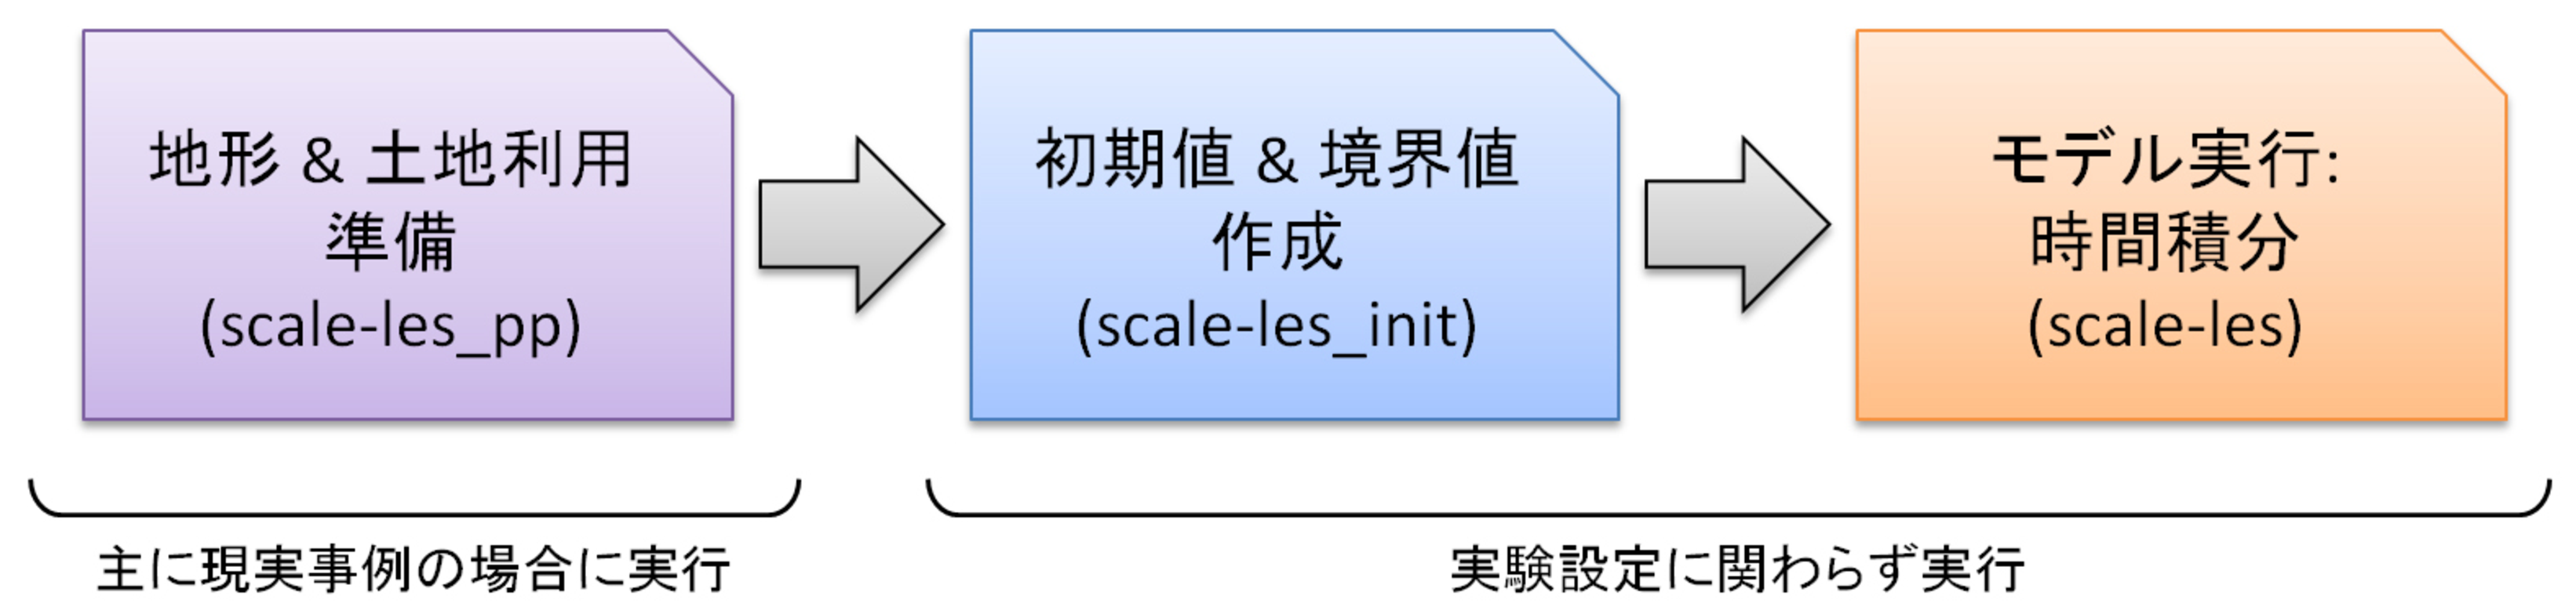
\includegraphics[width=0.9\hsize]{./figure/how_to_run.eps}\\
  \caption{SCALE-LESモデルの実行過程}
  \label{fig:howto}
\end{center}
\end{figure}



\subsection{チュートリアル:現実事例の実行方法}
%====================================================================================

ここでは,Fig. \ref{fig:domain}に示した日本域を対象とした実事例実験を行う.
計算領域(ドメイン)の設定はTable \ref{tab:grids}のようになっている.

\begin{figure}[t]
\begin{center}
  \includegraphics[width=0.5\hsize]{./figure/domain.eps}\\
  \caption{計算領域:コンターは海岸線,カラーシェードは地形の高度を示す.}
  \label{fig:domain}
\end{center}
\end{figure}

\begin{table}[t]
\begin{center}
  \caption{実験設定の概略}
  \label{tab:grids}
  \begin{tabularx}{150mm}{|l|X|} \hline
    \rowcolor[gray]{0.9} 項目 & 設定 \\ \hline
    水平格子数 (東西 x 南北) & 180格子点 x 180格子点 \\ \hline
    鉛直層数                 & 36層                  \\ \hline
    水平格子間隔             & dx = dy = 7500m       \\ \hline
    MPIプロセス分割 (東西 x 南北) & 3 x 3 (合計9プロセス) \\ \hline
    積分期間 & 1999年5月5日 00UTC~12UTC (12時間積分) \\ \hline
    時間ステップ間隔 & 30 sec (1440 steps) \\ \hline
  \end{tabularx}
\end{center}
\end{table}


\subsubsection{地形・土地利用データの作成:pp}
%-----------------------------------------------------------------------------------

ここでは,\ref{sec:source_code}節でダウンロードした\verb|tutorial_data|は,
\verb|${TOPDIR}|の下に展開されていると想定する.

まず,ppディレクトリへ移動する.\\
\begin{verbatim}
$ cd scale/scale-les/test/tutorial/pp
\end{verbatim}

ppディレクトリの中には,\verb|pp.conf|という名前のコンフィグファイルが準備されている.
地形・土地利用データを実験設定,およびSCALE-LESモデルの格子点に合わせたデータを
作成するために\verb|pp.conf|を編集するが,
チュートリアルでは,すでに編集済みの\verb|pp.conf|が与えられているためそのまま利用する.
\verb|pp.conf|の設定の中で特に注意するべき事は,\verb|PARAM_CONVERT|の項目である.

\begin{verbatim}
&PARAM_CONVERT
 CONVERT_TOPO = .true.,
 CONVERT_LANDUSE = .true.,
/
\end{verbatim}

上記のように\verb|CONVERT_TOPO|と\verb|CONVERT_LANDUSE|が\verb|.true.|となっていることが,
それぞれ地形と土地利用の処理を行うことを意味している.
詳細なコンフィグファイルの内容については,Appendix \ref{app:namelist}を参照されたい.


次に,コンパイル済みのバイナリと入力データをppディレクトリへリンクする.

\begin{verbatim}
$ ln -s ${TOPDIR}/scale/scale-les/test/tutorial/bin/scale-les_pp ./
$ ln -s ${TOPDIR}/tutorial_data/input_topo    ./
$ ln -s ${TOPDIR}/tutorial_data/input_landuse ./
\end{verbatim}


今回は,Table \ref{tab:grids}に示されているように,9つのMPIプロセスを使用する設定なので次のように実行する.
\begin{verbatim}
$ mpirun -n 9 ./scale-les_pp pp.conf
\end{verbatim}

正常にジョブが終了すれば,\verb|topo_d01.pe######.nc|と\verb|landuse_d01.pe######.nc|というファイルがMPIプロセス数だけ,つまり9つずつ生成される(\verb|######|にはMPIプロセスの番号が入る).
それぞれ,ドメインの格子点に内挿された地形と土地利用の情報が入ってる.

処理内容のログとして,\verb|pp_LOG_d01.pe000000|という名前でログファイルも出力されるので内容を確かめておくこと.
gpviewがインストールされていれば,次のコマンドによって作成された地形と土地利用データを描画してチェックすることができる.
正しく作成されていれば,Fig. \ref{fig:domain}と同じように描かれる.

\begin{verbatim}
$ gpview topo_d01.pe00000*@TOPO --aspect=1
$ gpview landuse_d01.pe00000*@FRAC_LAND --aspect=1
\end{verbatim}


\subsubsection{初期値・境界値データの作成:init}
%-----------------------------------------------------------------------------------

まず,initディレクトリへ移動する.\\
\begin{verbatim}
$ cd scale/scale-les/test/tutorial/init
\end{verbatim}

initディレクトリの中には,ppディレクトリと同様に\verb|init.conf|という名前のコンフィグファイルが準備されている.
チュートリアル用の\verb|init.conf|ファイルは,地球上でのドメインの位置や格子点数などは前節の設定にすでに合わせられている.
初期値・境界値データの作成には前節で作成した地形・土地利用データを利用するが,これは相対PATHを用いて参照するように設定されている.

\begin{verbatim}
&PARAM_TOPO
 TOPO_IN_BASENAME = "../pp/topo_d01",
/

&PARAM_LANDUSE
 LANDUSE_IN_BASENAME  = "../pp/landuse_d01",
/
\end{verbatim}


その他に\verb|init.conf|の設定の中で特に注意するべき事は,\verb|PARAM_MKINIT_REAL|の項目である.

\begin{verbatim}
&PARAM_MKINIT_REAL
 BASENAME_BOUNDARY   = "boundary_d01",
 FILETYPE_ORG        = "NICAM-NETCDF",
 NUMBER_OF_FILES     = 2,
 BOUNDARY_UPDATE_DT  = 21600.D0,
 INTERP_SERC_DIV_NUM = 20,
/
\end{verbatim}

このなかで\verb|BASENAME_BOUNDARY|は境界値データの出力名を指定している.
初期値データの出力名は別途\verb|PARAM_RESTART|の中の項目\verb|RESTART_OUT_BASENAME|で指定されている.
\verb|FILETYPE_ORG|は入力する気象場データのファイルフォーマットに関するパラメータを設定しており,
ここではNICAMモデルのnetcdf形式データのフォーマットで読み込むことを指定している.
\verb|NUMBER_OF_FILES|は読み込むファイルの数,\verb|BOUNDARY_UPDATE_DT|は読み込む入力データの
時間間隔をそれぞれ指定しており,最後の\verb|INTERP_SERC_DIV_NUM|は内挿計算用のチューニングパラメータである.
詳細なコンフィグファイルの内容については,Appendix \ref{app:namelist}を参照されたい.


次に,コンパイル済みのバイナリをinitディレクトリへリンクする.

\begin{verbatim}
$ ln -s ${TOPDIR}/scale/scale-les/test/tutorial/bin/scale-les_init ./
\end{verbatim}

入力データはinitディレクトリの中に準備されている,\verb|"inputdata-link.sh"|を用いてリンクする.
このスクリプトにあるstart dateとend dateの設定項目を実験設定に対応するように編集する.
ここでは,start dateは1999/05/05 00:00:00,end dateは1999/05/06 00:00:00と設定しておく.
もし,\verb|tutorial_data|を\verb|${TOPDIR}|以外の場所に展開している場合は,
\verb|"dir"|の項目も適切なディレクトリに変更すること.

\begin{verbatim}
$ sh inputdata-link.sh
\end{verbatim}
としてスクリプトを実行することで,気象場の入力データがリンクされ,initディレクトリ内に下記のファイルがリンクされる.

{\small \begin{verbatim}
la_tg_00000.peall.nc    ms_qv_00000.peall.nc   oa_sst_00000.peall.nc  ss_tem_sfc_00000.peall.nc
la_tg_00001.peall.nc    ms_qv_00001.peall.nc   oa_sst_00001.peall.nc  ss_tem_sfc_00001.peall.nc
la_wg_00000.peall.nc    ms_tem_00000.peall.nc  ss_q2m_00000.peall.nc  ss_u10m_00000.peall.nc
la_wg_00001.peall.nc    ms_tem_00001.peall.nc  ss_q2m_00001.peall.nc  ss_u10m_00001.peall.nc
lsmask_00000.peall.nc   ms_u_00000.peall.nc    ss_slp_00000.peall.nc  ss_v10m_00000.peall.nc
lsmask_00001.peall.nc   ms_u_00001.peall.nc    ss_slp_00001.peall.nc  ss_v10m_00001.peall.nc
ms_pres_00000.peall.nc  ms_v_00000.peall.nc    ss_t2m_00000.peall.nc
ms_pres_00001.peall.nc  ms_v_00001.peall.nc    ss_t2m_00001.peall.nc
\end{verbatim} }

さらに初期値・境界値データの作成過程ではモデルのほぼ全てのコンポーネントが起動される.
そのため陸面過程や放射過程のモデルを起動するためのパラメータファイルも用意しておく.

\begin{verbatim}
$ ln -s ${TOPDIR}/scale/scale-les/test/data/land/*  ./
$ ln -s ${TOPDIR}/scale/scale-les/test/data/rad/*   ./
\end{verbatim}
上の行のリンクコマンドによって陸面過程のパラメータファイルがリンクされ,
下の行のコマンドによって放射過程のパラメータファイルがリンクされる.


準備が整ったら,9つのMPIプロセスを使用してinitを実行する.
\begin{verbatim}
$ mpirun -n 9 ./scale-les_init init.conf
\end{verbatim}

正常にジョブが終了すれば,\verb|boundary_d01.pe######.nc|と\verb|init_d01_00010713600.000.pe######.nc|という
ファイルがMPIプロセス数だけ,つまり9つずつ生成される(\verb|######|にはMPIプロセスの番号が入る).
それぞれ,境界値データと初期値データが入ってるおり,境界値データには複数の時刻のデータが1つのファイルに含まれている.
初期値ファイルの名前のうち\verb|"00010713600.000"|の部分は,モデル内で算出された実験開始時刻を表している.

処理内容のログとして,\verb|init_LOG_d01.pe000000|という名前でログファイルも出力されるので内容を確かめておくこと.
gpviewがインストールされていれば,次のコマンドによって作成された地形と土地利用データを描画してチェックすることができる.
正しく作成されていれば,Fig. \ref{fig:init}と同じように描かれる.

\begin{verbatim}
$ gpvect --scalar --slice z=1500 --nocont --aspect=1 --range=0.001:0.015          \
         --xintv=10 --yintv=10 --unit_vect init_d01_00010713600.000.pe00*@QV      \
         init_d01_00010713600.000.pe00*@MOMX init_d01_00010713600.000.pe00*@MOMY
\end{verbatim}


\begin{figure}[t]
\begin{center}
  \includegraphics[width=0.7\hsize]{./figure/init_qv-momxy.eps}\\
  \caption{チュートリアル実験の初期場の様子:カラーシェードは高度1.5kmにおける水蒸気混合比の分布,ベクトルは高度1.5kmにおける水平運動量フラックスを表している.}
  \label{fig:init}
\end{center}
\end{figure}


\subsubsection{時間積分を行う:run}
%-----------------------------------------------------------------------------------

ここではいよいよSCALE-LESモデルを実行する.
まず,runディレクトリへ移動する.\\
\begin{verbatim}
$ cd scale/scale-les/test/tutorial/run
\end{verbatim}

runディレクトリの中には,これまでと同様に\verb|run.conf|という名前のコンフィグファイルが準備されている.
チュートリアル用の\verb|run.conf|ファイルは,ドメインの位置や格子点数などは前節の設定に合わせられている.
モデル本体の実行には事前に作成した地形・土地利用データや初期値・境界値データを利用するが,
これは相対PATHを用いて参照するように,それぞれ\verb|TOPO_IN_BASENAME|,\verb|LANDUSE_IN_BASENAME|,
\verb|RESTART_IN_BASENAME|,および\verb|ATMOS_BOUNDARY_IN_BASENAME|の項目で設定されている.

\begin{verbatim}
&PARAM_TOPO
 TOPO_IN_BASENAME = "../pp/topo_d01",
/

&PARAM_LANDUSE
 LANDUSE_IN_BASENAME  = "../pp/landuse_d01",
/

&PARAM_RESTART
 RESTART_OUTPUT      = .false.,
 RESTART_IN_BASENAME = "../init/init_d01_00010713600.000",
/

&PARAM_ATMOS_BOUNDARY
 ATMOS_BOUNDARY_TYPE        = "REAL",
 ATMOS_BOUNDARY_IN_BASENAME = "../init/boundary_d01",
 ATMOS_BOUNDARY_USE_VELZ    = .true.,
 ATMOS_BOUNDARY_USE_QHYD    = .false.,
 ATMOS_BOUNDARY_VALUE_VELZ  = 0.0D0,
 ATMOS_BOUNDARY_UPDATE_DT   = 21600.0D0,
/

\end{verbatim}


\verb|run.conf|の設定の中で時間積分に関する設定は,\verb|PARAM_TIME|の項目にある.

\begin{verbatim}
&PARAM_TIME
 TIME_STARTDATE             = 1999, 5, 5, 0, 0, 0,
 TIME_STARTMS               = 0.D0,
 TIME_DURATION              = 12.0D0,
 TIME_DURATION_UNIT         = "HOUR",
 TIME_DT                    = 30.0D0,
 TIME_DT_UNIT               = "SEC",
 TIME_DT_ATMOS_DYN          = 7.5D0,
 TIME_DT_ATMOS_DYN_UNIT     = "SEC",

 ~~中略~~

/
\end{verbatim}

\verb|TIME_STARTDATE|は時間積分を開始する時刻を設定する項目で,チュートリアルでは1999年5月5日0時UTCと設定する.
\verb|TIME_DURATION|は時間積分期間を設定する項目で,ここでは12時間積分を行う設定になっている.
最後に確認しておきたいのは,\verb|TIME_DT|,および\verb|TIME_DT_ATMOS_DYN|で,これらは時間積分の間隔(時間ステップ間隔:DT = Delta Time)を設定する項目である.前者は移流計算,後者はそれ以外の力学過程の計算に関する時間積分間隔である.
SCALE-LESモデルでは,そのほかの物理過程についても細かく時間積分間隔を設定できるようになっている.


出力データの設定である\verb|PARAM_HISTORY|も確認しておきたい.

\begin{verbatim}
&PARAM_HISTORY
 HISTORY_DEFAULT_BASENAME  = "history_d01",
 HISTORY_DEFAULT_TINTERVAL = 1800.D0,
 HISTORY_DEFAULT_TUNIT     = "SEC",
 HISTORY_DEFAULT_TAVERAGE  = .false.,
 HISTORY_DEFAULT_DATATYPE  = "REAL4",
 HISTORY_DEFAULT_ZINTERP   = .true.,
/
\end{verbatim}

\verb|HISTORY_DEFAULT_BASENAME|は出力するファイル名である.
\verb|HISTORY_DEFAULT_TINTERVAL|と\verb|HISTORY_DEFAULT_TUNIT|によってヒストリー出力時間間隔が設定される.
ここでは1800秒(30分)間隔での出力として設定されている.
この設定で,\verb|HISTITEM|として羅列された変数について出力される.

\begin{verbatim}
&HISTITEM item="DENS" /           ! density (3D)
&HISTITEM item="MOMZ" /           ! vertical momentum (3D)
&HISTITEM item="MOMX" /           ! horizontal momentum-x (3D)
&HISTITEM item="MOMY" /           ! horizontal momentum-y (3D)
&HISTITEM item="RHOT" /           ! density * potential-temperature (3D)

&HISTITEM item="QV"   /           ! mixing ratio for vapor (3D)
&HISTITEM item="QHYD" /           ! mixing ratio for hydrometeor (3D)

&HISTITEM item="T"    /           ! temperature (3D)
&HISTITEM item="PRES" /           ! pressure (3D)
&HISTITEM item="U"    /           ! horizontal wind component-x (3D)
&HISTITEM item="V"    /           ! horizontal wind component-y (3D)
&HISTITEM item="W"    /           ! vertical wind component (3D)
&HISTITEM item="PT"   /           ! potential temperature (3D)
&HISTITEM item="RH"   /           ! relative humidity (3D)

&HISTITEM item="PREC" /           ! precipitation (2D)
&HISTITEM item="OLR"  /           ! out-going longwave radiation

&HISTITEM item="U10" /            ! horizontal wind component-x at 10m height(2D)
&HISTITEM item="V10" /            ! horizontal wind component-y at 10m height(2D)
&HISTITEM item="T2"  /            ! temperature at 2m height (2D)
&HISTITEM item="Q2"  /            ! mixing ratio for vapor at 2m height (2D)

&HISTITEM item="SFC_PRES"   /     ! pressure at the bottom surface (2D)
&HISTITEM item="SFC_TEMP"   /     ! temperature a the bottom surface (2D)
&HISTITEM item="LAND_SFC_TEMP" /  ! temperature a the bottom surface for land model (2D)
&HISTITEM item="URBAN_SFC_TEMP" / ! temperature a the bottom surface for urban model (2D)

\end{verbatim}

たとえば,\verb|T|は温度(3次元変数),\verb|U|は水平風東西成分(3次元変数),
\verb|PREC|は積算地上降水量(2次元変数)などである.


その他に実験で使用される物理過程の設定は,\verb|PARAM_TRACER,PARAM_ATMOS,PARAM_OCEAN,PARAM_LAND,PARAM_URBAN|
の項目に記述されているので,実行前にチェックすること.
詳細なコンフィグファイルの内容については,Appendix \ref{app:namelist}を参照されたい.


次に,コンパイル済みのバイナリをrunディレクトリへリンクする.

\begin{verbatim}
$ ln -s ${TOPDIR}/scale/scale-les/test/tutorial/bin/scale-les ./
\end{verbatim}

また,前節と同様に陸面過程や放射過程のモデルを起動するためのパラメータファイルも用意しておく.

\begin{verbatim}
$ ln -s ${TOPDIR}/scale/scale-les/test/data/land/*  ./
$ ln -s ${TOPDIR}/scale/scale-les/test/data/rad/*   ./
\end{verbatim}
上の行のリンクコマンドによって陸面過程のパラメータファイルがリンクされ,
下の行のコマンドによって放射過程のパラメータファイルがリンクされる.


準備が整ったら,9つのMPIプロセスを使用してscale-lesを実行する.
\begin{verbatim}
$ mpirun -n 9 ./scale-les run.conf < /dev/null >&log&
\end{verbatim}


実行にはおおよそ2時間を要するため,上記のように標準出力をファイルへ
吐き出すようにしてバックグラウンドで実行しておくと便利である.
計算が開始されれば,処理内容のログとして,\verb|"LOG_d01.pe000000"|ファイルが生成されるので,
例えば下記のようなコマンドで\verb|"LOG_d01.pe000000"|ファイルを参照すれば,
どこまで計算が進んでいるかチェックすることができる.

\begin{verbatim}
$ tail -n 50 LOG_d01.pe000000
\end{verbatim}


正常にジョブが終了すれば,\verb|history_d01.pe######.nc|と\verb|restart_d01.pe######.nc|と
いう名前のファイルがMPIプロセス数だけ,つまり9つずつ生成される(\verb|######|にはMPIプロセスの番号が入る).
historyファイルは実行結果のプロダクトであり,restartファイルは対応する時刻を開始時刻として
再計算を開始するための初期値ファイルである.

次節でhistoryデータを描画して結果を調べる方法を説明する.


%####################################################################################

